IRSTI 20.15.05

\sectionwithauthors{А.Tynykulova, A.Mukhanova, A.Mukhomedyarova, A.Khamzina, Zh.Bagisov}{DEVELOPMENT AND APPLICATION OF AN INTEGRATED INFORMATION MODEL
FOR OPTIMIZING LAND USE AND FORECASTING YIELDS IN AGRICULTURAL
PRODUCTION}

\begin{center}
{\bfseries \textsuperscript{1,2}А.Tynykulova, \textsuperscript{1}A.Mukhanova, \textsuperscript{3}A.Mukhomedyarova, \textsuperscript{4}A.Khamzina, \textsuperscript{4}Zh.Bagisov}

\textsuperscript{1}L.N. Gumilyov Eurasian National University, Astana,
Kazakhstan,

\textsuperscript{2}Astana International University, Astana, Kazakhstan,

\textsuperscript{3} Zhangir Khan West Kazakhstan Agrarian and Technical
University, Uralsk, Kazakhstan,

\textsuperscript{4}M. Utemisov West Kazakhstan University, Uralsk,
Kazakhstan,

e-mail: asem\_110981@mail.ru,
\end{center}

The paper presents the development of a conceptual information model for
optimizing land use and crop forecasting in agriculture, implemented
using the PHP programming language, Javascript and the MYSQL database
management system. The model is designed to solve optimization problems
in various fields such as logistics, manufacturing, finance, etc.

As part of the work, an information model was developed, which is a set
of data, algorithms and software modules designed to solve optimization
problems. The model is implemented based on PHP, Javascript, and MYSQL
technologies.

The model allows you to solve optimization problems of varying
complexity using various optimization methods such as linear
programming, nonlinear programming, artificial intelligence methods,
etc.

The model can be applied to solve optimization problems in various
fields. In addition, the model allows you to solve optimization problems
with a high degree of accuracy and in a short time, and also has a
user-friendly interface that allows users to easily and quickly set
optimization tasks.

The current optimization problems and forecasting problems are not
covered in the work. How this will be implemented is not indicated in
the resulting information model.

The relevance of scientific research -- Every year farmers face the task
of how to use the land. And they face many factors, including
transportation costs, seed quality, cattle grazing and many other
options for using the land. But using the simulation model or
information system proposed by us, it is important to understand not
only the actual use of the land, but also the economic profit. The
system will indicate (advise) based on historical data as an expert,
what kind of crop to plant so that there is maximum benefit.
Agrotechnical indicators, allows you to create more accurate models and
forecasts, which contributes to making informed decisions. Such a system
allows farmers and agronomists to respond quickly to changing
conditions, optimize land use and improve the efficiency of agricultural
production in general.

An information model has been developed that will make it possible to
predict the harvest taking into account data on weather, soil, crops and
historical yield data, as well as optimize land use taking into account
data on soil type, climate, crop rotation and financial indicators. The
developed information model can improve the efficiency and
sustainability of agricultural production. The model can be used by
agronomists and farmers to make more informed decisions. The model takes
into account data on soil type, climate, crop rotation and financial
indicators to optimize land use.

{\bfseries Keywords:} information model, optimization, PHP, Javascript,
MYSQL, optimization tasks, logistics, production, economic profit.

\begin{center}
{\large\bfseries ЖЕРДІ ПАЙДАЛАНУДЫ ОҢТАЙЛАНДЫРУ ЖӘНЕ АУЫЛ ШАРУАШЫЛЫҒЫ
ӨНДІРІСІНДЕГІ ӨНІМДІЛІКТІ БОЛЖАУ ҮШІН ИНТЕГРАЦИЯЛАНҒАН АҚПАРАТТЫҚ
МОДЕЛЬДІ ӘЗІРЛЕУ ЖӘНЕ ҚОЛДАНУ}

{\bfseries \textsuperscript{1,2}А.Тынықұлова, \textsuperscript{1}А.
Мұханова, \textsuperscript{3}А. Мухомедьярова, \textsuperscript{4}А.
Хамзина, \textsuperscript{4}Ж.Багисов}

\textsuperscript{1}Л.Н. Гумилев атындағы Еуразия ұлттық университеті,
Астана, Қазақстан,

\textsuperscript{2}Астана халықаралық университеті, Астана, Қазақстан,

\textsuperscript{3}Жәңгір хан атындағы Батыс Қазақстан
аграрлық-техникалық университеті, Орал, Қазақстан,

\textsuperscript{4}М. Өтемісов атындағы Батыс Қазақстан университеті,
Орал, Қазақстан,

e-mail: asem\_110981@mail.ru
\end{center}

Жұмыста PHP бағдарламалау тілі, Javascript және MySQL дерекқорды басқару
жүйесі арқылы жүзеге асырылатын жерді пайдалануды оңтайландыру және ауыл
шаруашылығындағы егінді болжау үшін тұжырымдамалық ақпараттық модель
әзірлеу ұсынылған. Модель логистика, өндіріс, қаржы және т.б. сияқты
әртүрлі салалардағы оңтайландыру мәселелерін шешуге арналған.

Жұмыс аясында оңтайландыру мәселелерін шешуге арналған мәліметтер,
алгоритмдер мен бағдарламалық модульдер жиынтығы болып табылатын
ақпараттық модель жасалды. Модель PHP, Javascript, MySQL технологиялары
негізінде жүзеге асырылады.

Модель сызықтық бағдарламалау, сызықтық емес бағдарламалау, Жасанды
интеллект әдістері және т.б. сияқты әр түрлі оңтайландыру әдістерін
қолдана отырып, әр түрлі күрделілікті оңтайландыру мәселелерін шешуге
мүмкіндік береді.

Модельді әр түрлі салалардағы оңтайландыру мәселелерін шешу үшін
қолдануға болады. Сонымен қатар, модель оңтайландыру мәселелерін жоғары
дәлдікпен және қысқа мерзімде шешуге мүмкіндік береді, сонымен қатар,
пайдаланушыларға оңтайландыру тапсырмаларын оңай және жылдам орнатуға
мүмкіндік беретін ыңғайлы интерфейске ие. Модель жерді пайдалануды
оңтайландыру үшін топырақ түрі, климат, ауыспалы егіс және қаржылық
көрсеткіштер туралы деректерді ескереді.

Ауа райы, топырақ, дақылдар және тарихи кірістілік деректерін ескере
отырып, егінді болжауға, сондай-ақ, топырақ түрі, климат, ауыспалы егіс
және қаржылық көрсеткіштер туралы деректерді ескере отырып, жерді
пайдалануды оңтайландыруға мүмкіндік беретін ақпараттық модель
әзірленді. Әзірленген ақпараттық модель ауыл шаруашылығы өндірісінің
тиімділігі мен тұрақтылығын арттыра алады. Модельді агрономдар мен
фермерлер неғұрлым негізделген шешімдер қабылдау үшін қолдана алады

{\bfseries Түйін сөздер:} ақпараттық модель, оңтайландыру, PHP, Javascript,
MYSQL, оңтайландыру міндеттері, логистика, өндіріс, экономикалық пайда.

\begin{center}
{\large\bfseries Разработка и применение интегрированной информационной модели
для оптимизации землепользования и прогнозирования урожайности в
сельскохозяйственном производстве}

{\bfseries \textsuperscript{1,2}А.Тыныкулова,
\textsuperscript{1}А.Муханова, \textsuperscript{3}А.Мухомедьярова,
\textsuperscript{4}А.Хамзина, \textsuperscript{4}Ж. Багисов}

\textsuperscript{1}Евразийский национальный университет имени Л.Н.
Гумилева, Астана, Казахстан,

\textsuperscript{2}Международный университет Астана, Астана, Казахстан,

\textsuperscript{3} Западно-Казахстанский аграрно-технический
университет имени Жангир хана, Уральск, Казахстан,

\textsuperscript{4}Западно-Казахстанский университет им. М. Утемисова,
Уральск, Казахстан,

e-mail: asem\_110981@mail.ru
\end{center}

В работе представлена разработка концептуальной информационной модели
для оптимизации землепользования и прогнозирования урожая в сельском
хозяйстве, реализованная с использованием языка программирования PHP,
Javascript и системы управления базами данных MYSQL. Модель
предназначена для решения задач оптимизации в различных областях, таких
как логистика, производство, финансы и т.д.

В рамках работы была разработана информационная модель, которая
представляет собой совокупность данных, алгоритмов и программных
модулей, предназначенных для решения задач оптимизации. Модель
реализована на базе технологий PHP, Javascript, MYSQL.

Модель позволяет решать задачи оптимизации различной сложности,
используя различные методы оптимизации, такие как линейное
программирование, нелинейное программирование, методы искусственного
интеллекта и т.д.

Модель может быть применена для решения задач оптимизации в различных
областях. Кроме этого, модель позволяет решать задачи оптимизации с
высокой степенью точности и за короткое врем, а также имеет удобный
интерфейс, который позволяет пользователям легко и быстро задавать
задачи оптимизации. Модель учитывает данные о типе почвы, климате,
севообороте и финансовых показателях для оптимизации использования
земель.

Разработана информационная модель, которая позволит прогнозировать
урожай с учетом данных о погоде, почве, посевах и исторических данных о
урожайности, а также оптимизировать использование земель с учетом данных
о типе почвы, климате, севообороте и финансовых показателях.
Разработанная информационная модель может повысить эффективность и
устойчивость сельскохозяйственного производства. Модель может быть
использована агрономами и фермерами для принятия более обоснованных
решений

{\bfseries Ключевые слова:} информационная модель, оптимизация, PHP,
Javascript, MYSQL, задачи оптимизации, логистика, производство,
экономическая прибыль.

\begin{multicols}{2}
{\bfseries Introduction.} Over the past twenty years, land conflicts among
various land users have become more frequent. These conflicts have
devastating consequences for society, including the loss of lives and
the destruction of property {[}1{]}.

One of the main reasons for these conflicts is ineffective planning and
management of land resources. This can be caused by the use of
unsuitable tools and technologies for managing land cadasters {[}2{]}.

Information and communication technologies (ICT) can help solve this
problem. ICT tools such as Land Information Systems (LIS) and Geographic
Information Systems (GIS) can improve the planning and management of
land resources, thereby reducing the number of land conflicts.

Another factor contributing to land conflicts is the inefficiency in
providing land services. According to Mwaikambo and Hagai {[}3{]}, this
leads to delays in the registration of land rights and other problems.

The growth of the population and the increasing cost of land also
exacerbate the issue of land conflicts. The demand for land exceeds
supply, leading to disputes among various land users.

To address the problem of land conflicts, it is necessary to improve the
planning and management of land resources. Using ICT tools for land
cadaster management can create optimal conditions for enhancing the
efficiency of land service provision, as well as addressing issues
related to population growth and the rising cost of land.

Scientific novelty - For the first time an integrated model has been
proposed that combines data from agro-climatic conditions, soil
characteristics and agrotechnical measures for accurate forecasting of
yields and optimal distribution of land resources. New algorithms and
methods of big data processing have been developed, which can
significantly improve the accuracy of forecasts and the efficiency of
agricultural land use.

Undoubtedly, the issues discussed in this article are hypothetical, but
it is necessary to keep in mind that with the help of a conceptual
information model of land optimization and information flows, the needs
reflecting all sides of farmers\textquotesingle{} professional
activities can be identified. In our view, the basis of the conceptual
information model for agronomists should primarily lie in the objective
factors that influence the formation of their thematic structure.

These include the essence and tasks of the economic and social
development of the country, as well as agricultural policy, which
involves reorienting industry workers towards developing market
relations, increasing responsibility, and direct interest in the
rational use of production resources for necessary socio-economic
transformations. It is important to link these general tasks with the
specifics of a particular farm.

Information about the thematic structure of the
agronomists\textquotesingle{} information model for decision-making will
not be complete without studying the themes of needs of individual
peasant farms, conditioned by their private interests, the nature and
content of labor, specialization and area of crops, the presence of
temporary types of activities (folk crafts and crafts), as well as the
zonal characteristics of agricultural production.

To achieve success, a modern agronomist, as well as the head of a
peasant farm, must not only know the organizational and technological
processes of agricultural production but also be able to understand
issues of industry business, financing and accounting, marketing,
consumer demand, etc. For this, the most diverse information is needed,
presented not only in traditional periodicals and books of various kinds
but also in various automated information systems. Farmers, more than
other categories of agricultural production workers, are interested in
rapidly implementing the latest technologies in their farms. Information
modeling of land optimization should include not only objective factors
that affect their formation but also subjective factors, which, although
auxiliary, are important for organizing the solution.

An information model is an abstract representation of information that
describes its structure, connections, and interactions between elements.
It can be used to optimize various processes, including logistics,
production, and economic profit {[}4{]}.

Optimization is the process of finding the best solution or setting
parameters to achieve optimal results. In the context of the information
model, optimization may include improving performance, reducing costs,
or enhancing the efficiency of the system.

PHP, JavaScript, and MySQL. PHP is a programming language widely used
for developing web applications. It allows for the creation of dynamic
and interactive web pages {[}5, 6{]}.

JavaScript is a programming language used to create interactive elements
on web pages. It allows adding functionality, form validation,
animation, and other capabilities to web pages.

MySQL is a database management system used for storing and managing
data. It allows for the creation, modification, and retrieval of
information from the database.

Optimization in logistics and production may involve solving the
following tasks:

- Optimization of delivery routes: This task involves finding optimal
routes for delivering goods with minimal time and fuel costs.

- Optimization of inventory and warehouse management: This task involves
determining the optimal level of goods inventory at the warehouse to
minimize storage costs and avoid product shortages.

- Optimization of production processes: This task involves finding the
optimal production schedule to maximize resource use, reduce downtime,
and increase productivity.

Economic profit is the difference between total revenues and total costs
of a business. It is one of the main indicators of business efficiency
and success. Profit can be achieved by increasing revenues, reducing
costs, or a combination of both factors.

As technology advances, the accuracy and availability of information
models will only increase, leading to improved efficiency in
agricultural production and sustainable rural development.

{\bfseries Materials and methods.} The main research methods included
statistical methods, machine learning techniques, and data processing
software, as well as data processing software such as Python, R, and MS
Excel {[}7, 8, 9{]}.

The processing and analysis of statistical data include: data
collection; data cleaning; data transformation; data analysis; data
visualization.

An information model based on statistical data is able to predict crop
yields, which makes it possible to optimize the use of resources and
reduce risks. Using the model, it is possible to increase profitability
by implementing a project to increase profitability and environmental
efficiency.

As technology advances, the accuracy and accessibility of these models
will only increase, leading to increased agricultural production
efficiency and increased sustainability.

Methods of processing and analyzing statistical data involve not only
their collection, but also the study, processing and analysis. Like any
research, working with an information model begins with defining the
research problem and assessing its relevance {[}10{]}.

Optimizing the use of resources. The model allows not only to predict
the harvest, but also to optimize the use of resources such as water,
fertilizers, pesticides, and labor resources. This helps to reduce
costs, increase profitability and minimize the negative impact on the
environment.

Risk assessment. The model can help farmers assess the risks associated
with weather conditions, diseases and pests, as well as price
fluctuations in the market. This allows them to make more informed
decisions about the management of their farms.

Planning and decision-making. The model can be used to develop long-term
and short-term economic development plans. It can also help in making
operational decisions, for example, about the timing of sowing, watering
and harvesting.

Comparative analysis. The model allows you to compare productivity,
profitability and other key indicators of different farms, regions or
countries. This can help farmers identify best practices and improve
their work efficiency.

In addition to the above, information models based on statistical data
can be used for important activities and technological processes in
agriculture.

Development of new varieties and hybrids of agricultural crops. Models
can help breeders in the search for new varieties and hybrids with
higher yields, resistance to diseases and pests, as well as other
desirable traits.

Modeling of various scenarios. The models can be used to simulate
various scenarios of the future, for example, climate change, changes in
prices for agricultural products, and the introduction of new
technologies. This allows farmers to be prepared for possible changes
and plan their actions in advance.

Training and advising farmers. The models can be used to create training
materials and farmer counseling programs. This will help them improve
their knowledge and skills in using data to make better informed
decisions.

In general, statistical-based information models are a valuable tool for
improving the efficiency and sustainability of agricultural production.

The issues facing peasant farming include low productivity, inefficient
resource use, high risks, and food security, which is clearly
demonstrated in Figure 1.
\end{multicols}

\begin{figure}[H]
	\centering
	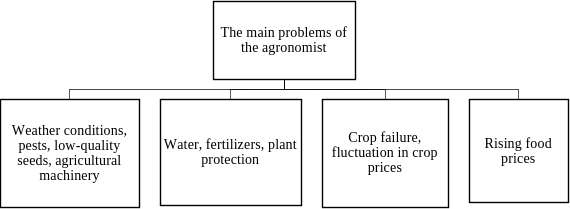
\includegraphics[width=0.6\textwidth]{assets/1002}
	\caption*{Figure 1 - The main problems of an agronomist (peasant economy)}
\end{figure}

\begin{multicols}{2}
All of the above factors influence the optimal use of land to build an
information model.

The materials are based on statistical data on the state of agricultural
lands on the example of the Ayyrtau district of the North Kazakhstan
region.

Table 1 shows data on weather conditions during the sowing period, which
shows the frequency of 15 days, which are divided into two columns, that
is, the dates 01.05 - 15.05 and 16.05 - 30.05.
\end{multicols}

\begin{table}[H]
\caption*{Table 1 - Statistical agrometeorological data for the last 5 years (data from the weather station of the village of Saumalkol in the Ayyrtau district of the North Kazakhstan region)}
\centering
\begin{tabular}{|r|l|rr|rr|rr|rr|rr|}
\hline
\multicolumn{1}{|l|}{\multirow{2}{*}{№}} & \multirow{2}{*}{Indicators} & \multicolumn{2}{r|}{2019}                                           & \multicolumn{2}{r|}{2020}                                           & \multicolumn{2}{r|}{2021}                                           & \multicolumn{2}{r|}{2022}                                           & \multicolumn{2}{r|}{2023}                                           \\ \cline{3-12}
\multicolumn{1}{|p{0.045\textwidth}|}{}                   &                             & \multicolumn{1}{p{0.045\textwidth}|}{01.05-15.05} & \multicolumn{1}{p{0.045\textwidth}|}{16.05-30.045} & \multicolumn{1}{p{0.045\textwidth}|}{01.05-15.05} & \multicolumn{1}{p{0.045\textwidth}|}{16.05-30.045} & \multicolumn{1}{p{0.045\textwidth}|}{01.05-15.05} & \multicolumn{1}{p{0.045\textwidth}|}{16.05-30.045} & \multicolumn{1}{p{0.045\textwidth}|}{01.05-15.05} & \multicolumn{1}{p{0.045\textwidth}|}{16.05-30.045} & \multicolumn{1}{p{0.045\textwidth}|}{01.05-15.05} & \multicolumn{1}{p{0.045\textwidth}|}{16.05-30.045} \\ \hline
1                                        & Temperature, 0C             & \multicolumn{1}{r|}{12}          & 13                               & \multicolumn{1}{r|}{18}          & 20                               & \multicolumn{1}{r|}{21}          & 22                               & \multicolumn{1}{r|}{20}          & 17                               & \multicolumn{1}{r|}{17}          & 20                               \\ \hline
2                                        & Precipitation, мм           & \multicolumn{1}{r|}{0,4}         & 0,3                              & \multicolumn{1}{r|}{0,8}         & 0                                & \multicolumn{1}{r|}{0}           & 0,2                              & \multicolumn{1}{r|}{1}           & 0                                & \multicolumn{1}{r|}{0,1}         & 0                                \\ \hline
3                                        & Air humidity, \%            & \multicolumn{1}{r|}{36}          & 40                               & \multicolumn{1}{r|}{43,5}        & 27,6                             & \multicolumn{1}{r|}{37,8}        & 39                               & \multicolumn{1}{r|}{36}          & 23                               & \multicolumn{1}{r|}{27}          & 30                               \\ \hline
4                                        & Wind speed, m/s             & \multicolumn{1}{r|}{2,6}         & 3                                & \multicolumn{1}{r|}{7,3}         & 4,6                              & \multicolumn{1}{r|}{6,1}         & 5,5                              & \multicolumn{1}{r|}{5,2}         & 4                                & \multicolumn{1}{r|}{7}           & 5,5                              \\ \hline
\end{tabular}%
\end{table}

\begin{multicols}{2}
It is during these dates that crops such as wheat, barley, corn and
alfalfa are actively sown in the area. We will not focus on any culture,
but data is important to us for further decision-making of the
information model. From Table 1, we see the average daily temperature,
humidity, etc. for favorable sowing.
\end{multicols}

\begin{table}[H]
\caption*{Table 2 - Statistical data on spring wheat crops in the Ayyrtau district of North Kazakhstan region over the past 5 years}
\centering
\begin{tabular}{|l|p{0.2\textwidth}|llllp{0.1\textwidth}|}
\hline
\multirow{2}{*}{№} & \multirow{2}{*}{Indicators}           & \multicolumn{5}{l|}{Sown area of spring wheat}                                                                                                                                                                                                                                                                                                                                                                                                              \\ \cline{3-7}
                   &                                       & \multicolumn{1}{l|}{2019}                                                                    & \multicolumn{1}{l|}{2020}                                                                            & \multicolumn{1}{l|}{2021}                                                                    & \multicolumn{1}{l|}{2022}                                                         & 2023                                                               \\ \hline
1                  & Date of sowing                        & \multicolumn{1}{l|}{05.05-15.05}                                                             & \multicolumn{1}{l|}{05.05-25.05}                                                                     & \multicolumn{1}{l|}{10.05-15.05}                                                             & \multicolumn{1}{l|}{05.05-20.05}                                                  & 05.05-20.05                                                        \\ \hline
2                  & Variety                               & \multicolumn{1}{p{0.1\textwidth}|}{Omsk 36 Akmola 2 Astana} & \multicolumn{1}{p{0.15\textwidth}|}{Omsk 36 Shortandinskaya 95 improved} & \multicolumn{1}{p{0.1\textwidth}|}{Omsk 36 Timas Asyl Sapa} & \multicolumn{1}{p{0.1\textwidth}|}{Omsk 36 Akmola 2} & Omsk 36 Virgin land 60 \\ \hline
4                  & The area of sowing, thousand hectares & \multicolumn{1}{l|}{276,4}                                                                   & \multicolumn{1}{l|}{282,1}                                                                           & \multicolumn{1}{l|}{290,3}                                                                   & \multicolumn{1}{l|}{295,7}                                                        & 301,2                                                              \\ \hline
\end{tabular}%
\end{table}

\begin{multicols}{2}
As we can see from Table 2, it takes a lot of time to process digital
data. The analysis of the table leads to the fact that there are several
varieties of spring wheat, and sowing proceeds in a chaotic, in our
opinion, random, unpredictable way.

But, experts in the field of agriculture, from table 1, analyze and
decide which variety to plant on a particular piece of land. Managing
such a complex process as farming, a decision that will lead to
considerable losses and losses, pushes us to develop an information
model for optimizing both costs and land use. Given the amount of
information for processing the model, we will divide it into subsystems:
crop programming and land optimization.

If the same crop is grown in the same field for many years in a row, the
harvest will get worse every year. In addition, plants will be overcome
by diseases and pests, and the soil will be depleted. Crop rotation of
crops involves the alternation of plants, and it is necessary to
alternate competently.

The information model of crop planning takes into account data on
weather, soil, crops and historical yield data, which allows us to
visually see the result in the form of yield values in tons {[}11,
12{]}. The general type of information flows is considered on the
example of a farm, in other cases, information flows occur according to
the same principle. A preview is shown in Figure 2.
\end{multicols}

\begin{figure}[H]
	\centering
	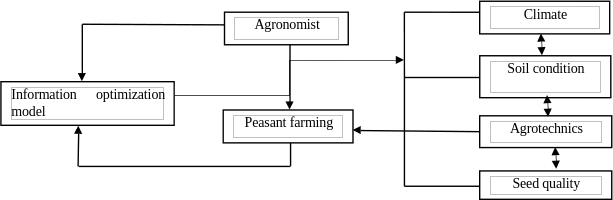
\includegraphics[width=0.6\textwidth]{assets/1003}
	\caption*{Figure 2 - General view of information flows}
\end{figure}

\begin{multicols}{2}
When developing an information model for optimizing agricultural land,
it is possible to identify the main factors affecting the efficiency and
economic profit of each site. 10 tables have been developed that provide
information on the storage of crop data, soil and climatic indicators.
The Laravel framework and Composer package manager are used to develop
the server part of the program, while the React library and npm package
manager are used for the client part of the program.

INSERT INTO Area (areaid, userid, arename, area) VALUES (NULL,
\textquotesingle1\textquotesingle, \textquotesingle111\textquotesingle,
\textquotesingle101\textquotesingle);

INSERT INTO User (userid, username, email, password) VALUES (NULL,
\textquotesingle Assemgul\textquotesingle,
\textquotesingle qwerty\textquotesingle).

Cannolly and Begg (2005) define conceptual database design as the
creation of an information model reflecting the activities of an
enterprise. This model does not depend on technical details, but it is
understandable to both end users and developers {[}13{]}. The authors
emphasize that the conceptual design stage begins with the development
of a conceptual data model that is completely separate from the
implementation details. This means that the model does not depend on the
target DBMS, application programs, programming languages, hardware
platform, performance issues and other technical aspects {[}14{]}. The
conceptual data model is documented using ER diagrams and a data
dictionary. Figure 3 shows an ER diagram of the LIS database data, which
shows entities, attributes, and relationships.
\end{multicols}

\begin{figure}[H]
	\centering
	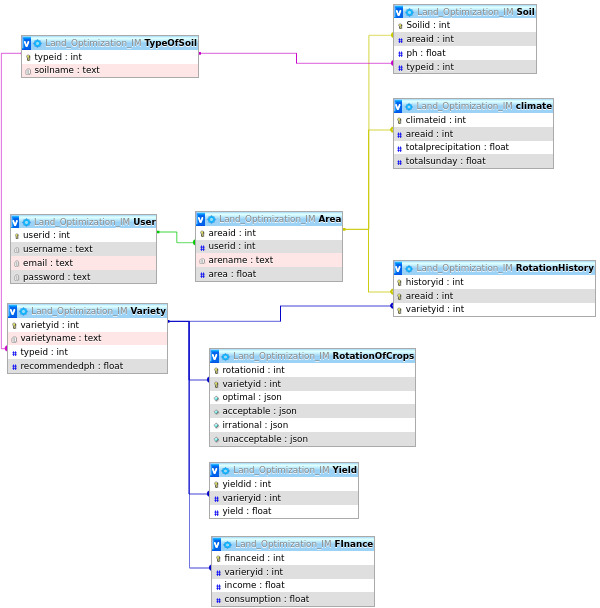
\includegraphics[width=0.8\textwidth]{assets/70}
	\caption*{Figure 3 - LIS database schema}
\end{figure}

\begin{multicols}{2}
Figure 3 illustrates the relationships between the tables of the system.
The research presented in the paper was aimed at studying user
requirements and developing the architecture of the proposed Land
management Information System (LIS). The study presents two
contributions. Firstly, the identified user requirements will help LIS
developers create systems that meet the real needs of users described in
{[}15, 16{]}.

Secondly, the paper presents the architecture of the proposed LIS, which
includes two main components: a component of land use allocation and an
assessment component. These components provide storage and extraction of
land use information, as well as storage, extraction and analysis of
estimated information. The purpose of the system is to improve the
efficiency and effectiveness of land management in the districts of
Tanzania. This is achieved by providing decision makers with accurate
data necessary for their work.

Accurate information and proper valuation of land plots, in turn,
contribute to improving revenue collection. After defining the
architecture of the platform and the rules of the association, it was
necessary to develop the software part of the web platform. The paper
presents the implementation of server rules in the Drools engine.

The server consists of three main components:

An application for registering data from external sensors in the system.
Devices or applications register as data sources by sending information
via a socket to the middleware. This software prepares data according to
the type of sensor.

2. The Drools rules module is the core of the server. It accepts the
prepared data, applies rules to it, and generates events.

3. Data warehouse -- a database that stores all the data used by the
system.

The development of a model that helps to use the land correctly takes
into account a number of factors. The materials are based on statistical
data on the state of the designated lands on the example of the Ayyrtau
district of the North Kazakhstan region. Continuous cultivation of one
crop in the same field leads to a decrease in yield, diseases and pests,
and soil depletion. Therefore, it is necessary to use crop rotation,
with the correct alternation of crops. The information model of crop
planning takes into account data on climate, soil, vegetation and other
factors.

{\bfseries Results and discussion.} The presented system is a web
application developed in the PHP language. It is designed to optimize
agricultural activities by collecting and analyzing data.

Figure 4 shows the structure of the database that is used in the system.
It contains information about weather conditions affecting agriculture,
the types of crops that can be grown in specific conditions, and the
financial situation of agricultural enterprises.
\end{multicols}

\begin{figure}[H]
	\centering
	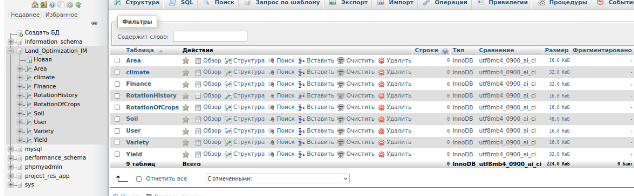
\includegraphics[width=0.9\textwidth]{assets/71}
	\caption*{Figure 4 - Sql database}
\end{figure}

\begin{multicols}{2}
The use of an optimization system makes it possible to increase the
efficiency of agricultural production, reduce the risks associated with
weather conditions and other factors, as well as increase the profits of
agricultural enterprises.

The presented system is a valuable tool for optimizing agriculture. It
allows farmers to make more informed decisions, which leads to increased
efficiency and profitability of their activities.

In general, the proposed information model will make it possible to
soberly assess the potential of agricultural lands, determine the
optimal land use options, and possibly increase the efficiency of
agricultural production. When developing the information model, such
factors as climate, land suitability, soil condition, legal and economic
aspects of the land were used. The statistical data used in the
information model over the past 5 years are mathematical in nature,
which is easy to calculate using mathematical methods.

After authenticating on the site and sending a request to the server.
The server calculates which cultures are similar to the sites of our
user and outputs them to the client side. According to the results of
testing the information model of the system, the following results were
recorded.
\end{multicols}

\begin{figure}[H]
	\centering
	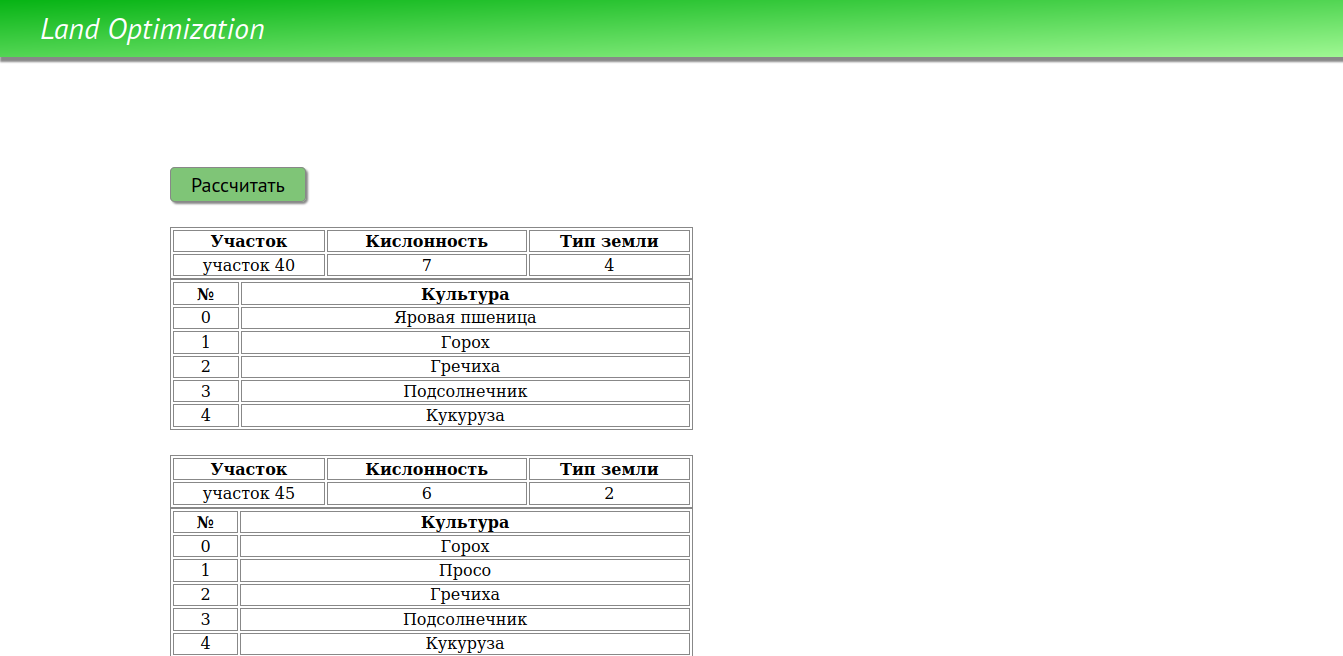
\includegraphics[width=0.9\textwidth]{assets/72}
	\caption*{Figure 5 - Scenario on the level of restrictions on sowing}
\end{figure}

\begin{multicols}{2}
The proposed system is a revolutionary tool that radically simplifies
the tasks of land use and assessment. It provides reliable and secure
storage for working with huge amounts of land data in real time.

The system\textquotesingle s compliance with all of the above criteria,
as well as the use of open data on agricultural land and the possibility
of involving agricultural experts in the development of the model, open
up wide opportunities for further research. This will allow the model to
be integrated with other information systems, which will lead to the
creation of an even more powerful and versatile tool.

One of the key advantages of the system is its ability to generate
graphs and diagrams that clearly demonstrate the dynamics of yields,
costs and revenues. This allows users to easily track changes in key
indicators and make informed decisions based on reliable data.

The implementation of the proposed system can have far-reaching
consequences for various sectors of the economy, including agriculture:
increasing yields, optimizing resource use, reducing production costs;
forestry: optimizing logging, preserving forest resources; real estate:
more accurate assessment of land value, improving the efficiency of land
asset management; environmental protection: combating land degradation,
conservation of biodiversity.

Thus, the proposed system is a powerful tool that can significantly
improve the efficiency of land management and contribute to the
sustainable development of the economy.

The implementation of the model is the launch of pilot projects in
different agro--climatic zones to test and adapt the system. Organizing
training for farmers and agronomists on the use of the system and
collecting feedback to improve it. Organizing training for farmers and
agronomists on the use of the system and collecting feedback to improve
it.

This approach will ensure the integrated and rational use of land
resources, increasing their productivity and sustainability of
agricultural production.

{\bfseries Conclusion.} In the course of our research, an information model
on crop rotation and crop optimization was developed for further
information processing and machine learning. Databases and the use of
SQL queries will make it easier to find the information that the farmer
needs. The developed web service, which uses the Django tool, can
download data and receive data processing if necessary. As a result, an
algorithm of agronomic farming was developed, which contains all the
information necessary for its management. But the result of the study
was a model that would make a decision when using land, and the best
option for its use. We believe that the developed information model of
crop rotation and crop optimization has great potential for improving
the efficiency of agronomic farming and ensuring food security.

This optimization model is implemented as a web service, which makes it
accessible to a wide range of users. It can be supplemented with modules
for crop forecasting, risk assessment, and inventory management. In
addition, the information model can be integrated with agricultural
enterprise management systems, meteorological services, and must also be
adapted to the climatic, soil and economic conditions of specific
regions.

The development of information systems to support decision-making in
agronomic farming is an urgent task of great importance for ensuring
food security. The proposed information model represents the first and
most general thematic expression of one of the current areas of activity
of automation of agricultural structures by software of the appropriate
level when making a decision. The model can be used by farmers to
increase the profitability of their farms and optimize the use of
resources.
\end{multicols}

\begin{center}
{\bfseries References}
\end{center}

\begin{noparindent}
1.Charity Mugabi Challenges Facing Land Ownership in Rural Tanzania:
What needs to be done?

ESRF Policy Brief.//Geography, Ecology, Economics, 2013.- No. 4

https://www.semanticscholar.org/paper/Challenges-Facing-Land-Ownership-in-Rural-Tanzania

2. A.P. Cherenkov Informacionnye sistemy dlja jekonomistov: ucheb.
posobie / Mosk. akad. jekonomiki i prava. -Moskva: Jekzamen, 2004.- 190
s. ISBN 5-94692-833-3 {[}in Russian{]}

3.Eric Mwaikambo, Martin Hagai. The Role of Land Information System in
Instigating Development of a National Spatial Data Infrastructure in
Tanzania //Conference FIG Working Week 2013. Environment for
Sustainability. - Abuja, Nigeria, 2013.-P.6-10.{[}Google Scholar{]}

4.Flanagan D. JavaScript: The Definitive Guide, 7th Edition.-2020. ISBN:
9781491952023.

https://www.oreilly.com/library/view/javascript-the-definitive/9781491952016/.

5.Forta B. MySQL: The Complete Reference. Crash Course 1st Edition.
https://www.amazon.com/MySQL-Crash-Course-Ben-Forta/dp/0672327120.

6. Homonenko A.D., Cygankov V.M., Mal\textquotesingle cev M.G. Bazy
dannyh. Uchebnik dlja vuzov - 4-e izdanie, dop. i pererab. - SPb.:
KORONA print. -- 2004. - 736 s. ISBN 5-7931-0284-1 {[}in Russian{]}

7.Emmanuel M. Falanta, Kenneth M.K. Bengesi. Drivers and Consequences of
Recurrent Conflicts between Farmers and Pastoralists in Kilosa and
Mvomero Districts, Tanzania/ Journal of Sustainable Development, 2018.-
Vol. 11( 4) -P. 13-26. https://doi.org/10.5539/jsd.v11n4p13. \hl{}

8. Vasil\textquotesingle ev A. Programmirovanie na RNR v primerah i
zadachah / Aleksej Vasil\textquotesingle ev. - Moskva: Jeksmo. // -2021.
-352 s. (Rossijskij komp\textquotesingle juternyj bestseller). ISBN
978-5-04-122022-8. {[}in Russian{]}

9. Malyhina M.P. Bazy dannyh: osnovy, proektirovanie,
ispol\textquotesingle zovanie. /BHV-Peterburg. -- 2007. - 528 s. ISBN:
978-5-94157-941-9. {[}in Russian{]}

10. Petrov V.N. Informacionnye sistemy: Ucheb. dlja vuzov. /Piter. --
2002. - 688 s. ISBN 5-318-00561-6. {[}in Russian{]}

11. Rizalino B. Cruz. Developing Land Information System for local
government: the case of Naga city Philippines.// -200. --P.114.

https://www.muthar-alomar.com/wp-content/uploads/2013/01/Landuse-Info.-System.pdf

12.Robin McLaren, United Kingdom Can the Innovative Use of Mobile Phones
Support More Effective Land Administration Services? //XXIV FIG
International Congress 2010 Facing the Challenges - Building the
Capacity. - Sydney, Australia, 2010. -P. 12-24.

13. Sibiljov V.D. Bazy dannyh: Metodicheskie ukazanija po vypolneniju
samostojatel\textquotesingle noj i individual\textquotesingle noj raboty
studentov dlja napravlenija podgotovki bakalavra 230100.62 - Informatika
i vychislitel\textquotesingle naja tehnika. Profil\textquotesingle{} -
Programmnoe obespechenie sredstv vychislitel\textquotesingle noj tehniki
i avtomatizirovannyh system -Tomsk: TUSUR, 2013, -7 s. {[}in Russian{]}

14.Thomas Connolly, Carolyn Begg. Database systems. A practical approach
to design, implementation and management. Pearson Education Limited.
England.// -2015. -1255 P.

ISBN 13: 978-1-292-06118-4.

15.Rick F., Van der Lans. SQL for MySQL developers: A comprehensive
tutorial and reference. // Addison-Wesley Professional, 2007.-1037 P.
ISBN 978-0-13-149735-1.

16.Nicholas C. Zakas High Performance JavaScript: Build Faster Web
Application Interfaces: 1st Edition// Yahoo Press, 2012.-232P. ISBN:
978-5-93286-213-1.
\end{noparindent}

\emph{{\bfseries Information about the authors}}

\begin{noparindent}
Tynykulova A.S. - doctoral student of the L.N. Gumilyov Eurasian
National University, Master of Computer Science, Senior Lecturer of the
Astana International University, Astana, Kazakhstan, e-mail:
asem\_110981@mail.ru;

Mukhanova A.A. - PhD, associate professor L.N. Gumilyov Eurasian
National University, Astana, Kazakhstan, е-mail: ayagoz198302@mail.ru;

Mukhomedyarova A.S. - Associate Professor, PhD, Zhangir Khan West
Kazakhstan Agrarian and Technical University, Uralsk, Kazakhstan,
Institute of Agrotechnology, e-mail: aina25111980@mail.ru;

Khamzina A.A. - Senior lecturer, Head of educational programs for the
training of computer science teachers and IT specialists, M. Utemisov
West Kazakhstan University, Uralsk, Kazakhstan, e-mail:
akmaral\_abilk@mail.ru;

Bagisov Zh.Zh. - Master, doctor of DBA, M. Utemisov West Kazakhstan
University, Uralsk, Kazakhstan, e-mail: Bag\_8585@mail.ru.
\end{noparindent}

\emph{{\bfseries Сведения об авторах}}

\begin{noparindent}
Тыныкулова А.С. - докторант Евразийского национального университета им.
Л.Н. Гумилева, магистр информатики, старший преподаватель Международного
университета Астана, Астана, Казахстан,

e-mail: asem\_110981@mail.ru;

Муханова А.А. - PhD, ассоциированный профессор, Евразийский национальный
университет им. Л.Н. Гумилева, Астана, Казахстан, е-mail
ayagoz198302@mail.ru;

Мухомедьярова А.С. - PhD, доцент, Западно-Казахстанский
аграрно-технический университет им. Жангир хана, Уральск, Казахстан,
институт агротехнологий, e-mail: aina25111980@mail.ru;

Хамзина А.А. - старший преподаватель, руководитель образовательных
программ по подготовке учителей информатики и IT-специалистов,
Западно-Казахстанский университет им. М. Утемисова, Уральск, Казахстан,
e-mail: akmaral\_abilk@mail.ru;

Багисов Ж.Ж. - магистр, доктор DBA, Западно-Казахстанский университет
им. М. Утемисова, Уральск, Казахстан, e-mail: Bag\_8585@mail.ru.
\end{noparindent}
